\documentclass[conference]{IEEEtran}
\IEEEoverridecommandlockouts
\usepackage{amsmath,amssymb,amsfonts,algorithmic,graphicx, textcomp, cite, xcolor, algorithm2e, hyperref}
\DeclareMathOperator*{\argmin}{arg\,min}
\def\BibTeX{{\rm B\kern-.05em{\sc i\kern-.025em b}\kern-.08em
		T\kern-.1667em\lower.7ex\hbox{E}\kern-.125emX}}
\newcounter{mytempeqncnt}
\begin{document}

	\title{Efficient Hessian-Free Optimization of \\Deep Neural Networks}


	\author{\IEEEauthorblockN{Niklas Brunn}
		\IEEEauthorblockA{\textit{Albert Ludwigs University of Freiburg} \\
			\textit{Mathematical Institute}\\
			Freiburg, Germany \\
			niklasbrunn@web.de}
		\and
		\IEEEauthorblockN{No\"{e}l E. Kury}
		\IEEEauthorblockA{\textit{Albert Ludwigs University of Freiburg} \\
			\textit{Mathematical Institute}\\
			Freiburg, Germany \\
			nekury@wkury.de}
		\and
		\IEEEauthorblockN{Clemens A. Schächter}
		\IEEEauthorblockA{\textit{Albert Ludwigs University of Freiburg} \\
			\textit{Mathematical Institute}\\
			Freiburg, Germany \\
			clemens.schaechter@live.com}
	}

	\maketitle
	\thispagestyle{plain}
	\pagestyle{plain}

	\begin{abstract}
		\noindent
		This report is a written elaboration of a project which was developed in the lecture Numerical Optimization in the winter term 21/22 at the Albert Ludwigs University of Freiburg.\\
		We discuss a $2^{\text{nd}}$-order optimization method for training deep neural networks using the generalised-Gauss Newton Matrix as an approximation for the Hessian of the objective loss function. In addition we present an implementation of the method using Python3, Tensorflow and compare the results to a $1^{\text{st}}$-order optimization method on the MNIST dataset.
	\end{abstract}

	\section{Introduction}
	\noindent
	Deep neural networks (DNNs) are an important deep learning architecture and have a wide field of applications. When training a DNN, the network parameters are updated according to certain rules, which we call the DNN optimization method. Here stochastic gradient descent (SGD) is often used as such an optimization method. SGD is a $1^{\text{st}}$-order optimization method in which only the negative gradient of the objective loss function (OL) with respect to the network parameters is used to update the current parameters. One problem of SGD is that pathological curvature of the OL is not considered. This means that the method can get stuck in saddle points, or often converges very slowly in enviroments with pathological curvature.\\
	On the other hand $2^{\text{nd}}$-order optimization methods take into account the curvature of the OL and can thus circumvent such problems. But they are often costly in time because $2^{\text{nd}}$-order derivatives must be computed for this purpose.\\
	Our aim is to use a version of Newton's method for DNN optimization as presented in [4]. We use an approximation of the Hessian matrix, which is positive definite, and thus allows the use of a preconditioned version of the conjugate gradient (PCG) method for updating the network parameters. Therefore we discuss the individual problems of standard Newton updates and the improvements proposed for them in order to ensure computational efficiency. Our own implementation can be accessed on GitHub \href{https://github.com/NiklasBrunn/Hessian_Free_Optimization_of_Deep_Neural_Networks}{(GitHub repository)}.\\
	Finally we train a DNN on the MNIST-dataset with SGD and the here presented $2^{\text{nd}}$-order optimization method and discuss our results.


	\section{Optimization of Deep Neural Networks}
	\noindent
	In this section, we introduce the necessary mathematical notations for optimizing DNNs, formulate the parameter optimization task as a nonlinear programmming problem (NLP) and explain tricks for the OL, that will be useful in the implementation of the presented optimization method.

	\subsection{Deep Neural Networks}
	\noindent
	A deep neural network is an artificial neural network in which additional layers between input and output layer provide some depth. Given a dataset consisting of observation pairs $D =\{(x_{i}, y_{i})\}_{1\leq i\leq N}$ with inputs $x_{i}$ and corresponding targets $y_{i}$, we aim to find a set of parameters so that the DNN's evaluations are approximately the corresponding observed targets $y_{i}$.\\
	In contrast to standard convention we define the realisation of a DNN given a fixed input $x$ as
	\begin{align}
	&R_{x}:\Theta^{d}\rightarrow\mathbb{R}^{m}, \notag\\
	&\theta\mapsto R_{x}(\theta) =: z_{x}.
	\end{align}
	Here $\theta$ is a vector containing the parameters of our DNN and $z_{x}$ is defined as the DNN's output vector. The parameter space is denoted by $\Theta^{d} := \mathbb{R}^{d}$ with usually $d>>0$. More precisely the realisation is an alternating concatenation of a fixed number of affine and nonlinear mappings with respect to its input $x$. The parameter vector is the collection of every entry from all weight matrices and bias vectors in the affine mappings. These affine mappings are called layers and the nonlinear mappings are called activation functions. Activation functions $\varrho:\mathbb{R}\rightarrow\mathbb{R}$ are one-dimensional, nonlinear, real-valued and piecewise differentiable functions which are applied element-wise to the activation of the preceding layer. Usually the same activation function is applied to all hidden layers of the DNN. We assume that an additional nonlinear function $\phi:\mathbb{R}^{m}\rightarrow\mathbb{R}^{m}$ is applied to the DNN's output which is not directly considered as a component of the DNN's architecture. This allows us to use technical tricks that later favor the implementation. We denote the nonlinear evaluation of the network output by
	\begin{align}
	\hat{y}_{x} := \phi(z_{x}),
	\end{align}
	which serves as an approximation to the target $y$. We also allow $\psi$ to be the identity function for cases in which no further mapping of the network output is needed.


	\subsection{Loss functions}
	\noindent
	Choosing a good Loss function
	\begin{align}
	&L:\mathbb{R}^{m}\times \mathbb{R}^{m}\rightarrow \mathbb{R}^{+}, \notag\\
	&(\hat{y}, y)\mapsto L(\hat{y}, y).
	\end{align}
	is an important task in parameter optimization of DNNs. The Loss is a feedback about how well the DNN fits the observation data set. Further we define the output loss function given a fixed target $y$ as
	\begin{align}
	&L_{y}:\mathbb{R}^{m}\rightarrow \mathbb{R}^{+}, \notag\\
	&\hat{y}\mapsto L_{y}(\hat{y}) := L(\hat{y}, y),
	\end{align}
	which is assumed to be at least twice continous differentiable in $\hat{y}$. The output loss takes $\hat{y}_{x} = \phi(R_{x}(\theta))$ as input for a fixed observation pair $(x, y)$ with current parameters $\theta$. A typicall choice for the loss function $L$ and the previous nonlinear function $\psi$ in multi-classification tasks is crossentropy loss with softmax function and squared error loss with identity function for regression tasks.



	\subsection{Network training formulated as a NLP}
	\noindent
	Parameter optimization of a DNN can be formulated as an unconstrained NLP. Therefore we define the OL as a mapping which calculates the empirical risk of the DNN`s output with current parameters $\theta$ given the observation data set
	\begin{align}
	&f_{D}:\Theta^{d}\rightarrow\mathbb{R}^{+}, \notag\\
	\theta\mapsto f_{D}(\theta) &:= \mathbb{E}_{D}[L_{y}(\hat{y}_{x})] =  \frac{1}{N}\sum_{j = 1}^{N}L_{y_{j}}(\hat{y}_{x_{j}}).
	\end{align}
	Thus we get the unconstrained NLP formulation
	\begin{align}
	\argmin_{\theta\in\Theta^{d}}\quad f_{D}(\theta),
	\end{align}
	where $\theta$ denotes the decision variable and $f_{D}$ the objective function of the NLP.
	Further, if we consider only one observation $(x, y)$ from the observation data set $D$, we simply write  $f$ for the corresponding OL. Note that the above formulated NLP is typically nonconvex due to the nonconvexity of the OL.

	\subsection{Matching loss functions}
	\noindent
	For later purposes we need to calculate the Jacobian or the gradient of the OL with respect to the DNN`s parameters. For simplicity we consider the OL for only one pair of observations
	\begin{align}
	J_{f} := \frac{\partial}{\partial\theta}f(\theta)
	\end{align}
	and in the notation neglect the dependency to the parameters $\theta$ to ensure readability.
	The results can be extended without problems to the case where the whole data set or a batched version of the whole data set is considered due to linearity of the derivative.
	Applying the chain rule we can rewrite the Jacobian in (7) to
	\begin{align}
	J_{f} &= J_{L_{y}\circ \:\phi \:\circ\:R_{x}} = J_{L_{y}} J_{\phi} J_{R_{x}},\\
	J_{f}^{\mathrm{T}} &= J_{R_{x}}^{\mathrm{T}}  J_{\phi}^{\mathrm{T}}  J_{L_{y}}^{\mathrm{T}}.
	\end{align}
	As introduced in [8], we also make use of so-called matching loss functions. An output loss function $L_{y}$ matches the output nonlinearity $\phi$ iff
	\begin{align}
	\left(\frac{\partial}{\partial\hat{y}_{x}}\left(L_{y}\circ \phi\right)(\hat{y}_{x})\right)^{\mathrm{T}}= J_{L_{y}\circ \:\phi}^{\mathrm{T}} = A z_{x} + b,
	\end{align}
	for a matrix $A$ and a vector $b$, which both do not depend on the network parameters $\theta$.\\
	Note that crossentropy loss matches the softmax function and squared error loss matches the identity function.


	\section{Hessian-Free optimization method}
	\noindent
	In this section we want to provide the reader a compact summary of the different components used in the presented optimization method. We will briefly review Newton`s method and discuss the advantages and disadvantages of the usage of the Hessian matrix and then introduce the necessary theory for the efficient $2^{\text{nd}}$-order optimization method called Hessian-Free method. For a more detailed introduction in Newton-type optimization we refer the reader to chapter 7 in [2]. For details about problems with pathological curvature to [4], and for informations about the generalised Gauss-Newton matrix to chapter 8 in [5].\\
	A pseudocode for the full Hessian-Free algorithm is given in Algorithm 1 (note that we use the positive gradient in the CG method and thus have to adapt the algorithm).

	\RestyleAlgo{ruled}
	\begin{algorithm}
		\SetKwInOut{Input}{Input}
		\SetKwInOut{Output}{Output}
		\SetKw{CG}{\textbf{pre.-CG($B,\:\Delta\theta_{k},\:J_{f}^{\mathrm{T}}(\theta_{k}),\:\lambda$):}}
		\SetKwInOut{LAM}{\textbf{$\lambda$-update($B,\: \Delta\theta_{k+1},\: \lambda$)}}
		\caption{Hessian-Free pseudocode for (6)}\label{alg:two}
		\KwIn{$D,\: \theta_{0},\: \lambda,\: \text{epochs}$}
		$\Delta\theta_{0}\gets 0$\\
		$k, e\gets 0$\\
		\While{$e< \mathrm{epochs}$}{
			$\mathbf{shuffle }\ D$\\
			\For{$\mathrm{Batch}\: B$ $\mathbf{in}$ $D$}{
				$\mathbf{compute}\: J_{f_{B}}^{\mathrm{T}}(\theta_{k})\:\text{with }\mathbf{BAD}$\\
				$\Delta\theta_{k+1}\gets \mathbf{PCG}(B,\:\Delta\theta_{k},\:J_{f_{B}}^{\mathrm{T}}(\theta_{k}),\:\lambda)$\\
				$\theta_{k+1}\gets \theta_{k} - \Delta\theta_{k+1}$\\
				$\lambda\gets \mathbf{\lambda}\text{-}\mathbf{update}(B,\: \Delta\theta_{k+1},\: \lambda)$\\
				$k\gets k+1$
			}
			$e\gets e+1$
		}
		\KwOut{$\theta^{\star}$}
	\end{algorithm}


	\subsection{Newton's method}
	\noindent
	Newton`s method is an optimization method, where we update the decision variables of our NLP formulation in (6) iteratively by
	\begin{align}
	\theta_{k+1} = \theta_{k} -H_{f}(\theta_{k})^{-1} J_{f}^{\mathrm{T}}(\theta_{k}),
	\end{align}
	where $H_{f}(\theta_{k})$ denotes the Hessian of the OL with respect to the current network parameters $\theta_{k}$. One can obtain this by minimizing the local quadratic approximation
	\begin{align}
	\text{ }\Delta\theta_{k+1} &:= \theta_{k+1} - \theta_{k},\\
	q_{\theta_{k}}(\Delta\theta_{k+1})&:= f(\theta_{k}) + J_{f}^{\mathrm{T}}(\theta_{k})\Delta\theta_{k+1} + \notag\\
	&\:\:\:\:\:\:\:\frac{1}{2}\Delta\theta_{k+1}^{\mathrm{T}}H_{f}(\theta_{k})\Delta\theta_{k+1}\\
	&\text{ }\approx f(\theta_{k} + \Delta\theta_{k+1}),
	\end{align}
	with respect to $\Delta\theta_{k+1}$. \\
	Using Newton's method can lead to convergence in fewer iterations than gradient descent. This is because it rescales the gradient of the OL in every step by using informations about the local curvature of the OL. This makes Newton's method less susceptible to pathological curvature, where $1^{\text{st}}$-order gradient based methods like SGD can get stuck in saddle points. We will also neglect the dependency on the parameters $\theta$ in our notation of the Hessian and Hessian approximations, whenever the matrix is not mentioned in the context of a Newton step.


	\subsection{Problems with the Hessian}
	\noindent
	We implicitly asume in every step (11) that the Hessian is invertible, which sometimes is not the case in our task (6). Since the Hessian is not necessarily positive semidefinite either, convergence to a local minimum can not be ensured. Furthermore the Hessian has $d^{2}$ entries consisting of $2^{\text{nd}}$-order partial derivatives, which makes it expensive to calculate, assuming $d>>0$. For these reasons, the direct application of Newton's method to our task is inappropriate and has to be modified to ensure an efficient application.

	\subsection{The generalized Gauss-Newton Matrix}
	\noindent
	We no longer use the Hessian itself, but the generalized Gauss-Newton matrix (GGN) as an approximation of the Hessian
	\begin{align}
	G_{f} := J_{R_{x}}^{\mathrm{T}}H_{L_{y}\circ\:\phi}J_{R_{x}},
	\end{align}
	where $H_{L_{y}\circ\:\phi}$ denotes the Hessian of $L_{y}\circ\:\phi$ with respect to $z_{x}$. The matrix $J_{R_{x}}$ denotes the Jacobian of the realisation of the DNN with respect to its parameters.
	Regarding the full Hessian of the OL
	\begin{align}
	H_{f} = J_{R_{x}}^{\mathrm{T}}H_{L_{y}\circ\:\phi}J_{R_{x}}\:\sum_{j = 1}^{m}\left(\left(J_{L_{y}\circ \:\phi}^{\mathrm{T}}\right)_{j} H_{(R_{x})_{j}}\right),
	\end{align}
	where $H_{(R_{x})_{j}}$ denotes the Hessian of the DNN`s  $j$-th output, the last sum-term in (16) vanishes if one of the two factors in the sum vanishes.
	This means that in a neighborhood of a local optimum $\theta^{\star}$ it holds that $H_{f} \approx G_{f}$.   Moreover, by construction, the GGN is symmetric and positive semidefinite if $L_{y}\circ\:\phi$ is convex, since for every $v\in\mathbb{R}^{d}$ it holds that
	\begin{align}
	v^{\mathrm{T}}G_{f}v &= v^{\mathrm{T}}\left( J_{R_{x}}^{\mathrm{T}}H_{L_{y}\circ\:\phi}J_{R_{x}}\right)v\\
	&= \left(J_{R_{x}}v\right)^{\mathrm{T}}H_{L_{y}\circ\:\phi}\left(J_{R_{x}}v\right) \\
	&\geq 0.
	\end{align}
	For both crossentropy loss with previous softmax function and sqared error loss with previous identity function it holds that $L_{y}\circ\:\phi$ is convex.

	\subsection{Levenberg-Marquardt algorithm }
	\noindent
	To ensure invertibility we use a damped version of the GGN (DGGN). The idea is to use a Levenberg-Marquardt algorithm, where we add a diagonal matrix with positive values on the diagonal, e.g.
	\begin{align}
	DG_{f} := G_{f} + \lambda\cdot I_{d},
	\end{align}
	with $I_{d}$ denoting the $d\times d$ unit matrix and some $\lambda>0$.
	The DGGN constructed this way is always positive definite.
	To see this, we consider the decomposition
	\begin{align}
	G_{f} = U\Lambda U^{\mathrm{T}},
	\end{align}
	with an orthogonal Matrix $U\in\mathbb{R}^{d\times d}$ containing the eigenvectors to the corresponding eigenvalues as colums and a diagonal Matrix $\Lambda\in\mathbb{R}^{d\times d}$ which on the diagonal entries contains the nonnegative eigenvalues of the GGN. This decomposition exists because the GGN is symmetric and positive semidefinite. Further it holds that
	\begin{align}
	DG_{f} &= U\Lambda U^{\mathrm{T}} + \lambda\cdot I_{d}\\
	&= U\Lambda U^{\mathrm{T}} + \lambda\cdot U I_{d}U^{\mathrm{T}}\\
	&= U\left(\Lambda + \lambda\cdot I_{d}\right)U^{\mathrm{T}},
	\end{align}
	where the Matrix $\left(\Lambda + \lambda\cdot I_{d}\right)$ is a diagonal one containing only positive entries, the eigenvalues, on the diagonal. Due to symmetry and because of the fact that the DGGN has only positive eigenvalues it holds that this matrix is positive definite and invertible.\\
	Note that a choice of $\lambda>>0$ leads to a Newton step where the change of our parameters is marginal. On the other hand $\lambda\approx 0$ leads to a full step using the GGN. In practice, we update the damping value $\lambda$ after each iteration. For this reason, the damping parameter can be seen as a self-adapting learning rate for the optimization method.\\
	Following [4] we define the reduction ratio
	\begin{align}
	\rho := \frac{f(\theta_{k}) - f(\theta_{k+1})}{q_{\theta_{k}}(\Delta\theta_{k + 1}) - q_{\theta_{k}}(0)}
	\end{align}
	and then update the value $\lambda$ according to the rule
	\begin{align}
	&\textbf{if}\:\rho<\frac{1}{4}:\notag\\
	&\text{ }\text{ }\text{ }\text{ }\lambda_{k+1} = r\cdot\lambda_{k}\notag\\
	&\textbf{elif}\:\rho>\frac{3}{4}:\notag\\
	&\text{ }\text{ }\text{ }\text{ }\lambda_{k + 1} = r^{-1}\cdot\lambda_{k}\notag\\
	&\textbf{else}: \notag\\
	&\text{ }\text{ }\text{ }\text{ }\lambda_{k + 1} = \lambda_{k}\notag\\
	&\textbf{return}:\:\lambda_{k + 1},
	\end{align}
	where $r=1.5$. We can compute the denominator of $\rho$ within the PCG-run and thus save some computation time (output denom in Alogrithm 2). Otherwise we need to compute an additional matrix-vector-product.\\
	In our experiments we found that for a smaller batch size (e.g. $N<150$) it is important to adjust the update amount of the damping value to a smaler size, e.g. $r=1.01$, to ensure stable convergence (see Fig. 1.). For a large batch size $r=1.01$ leads to slower convergence.

	\begin{figure}[htbp]
		\centerline{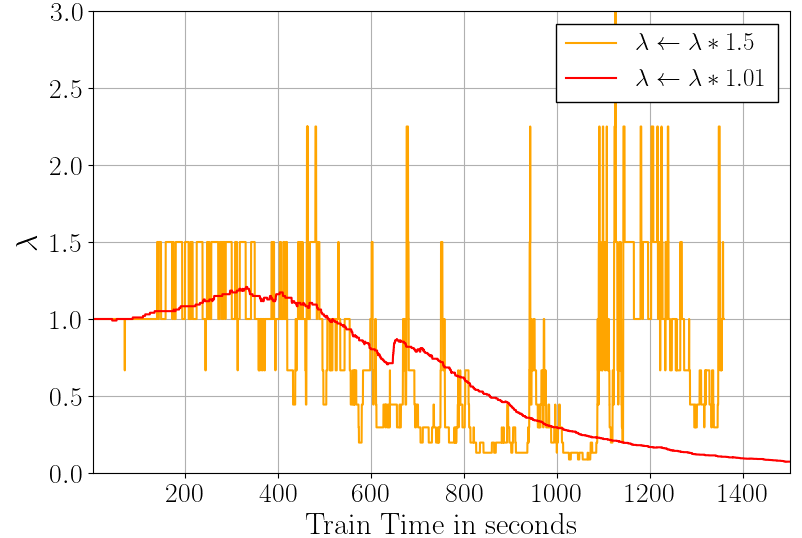
\includegraphics[scale=0.52]{lambda.png}}
		\caption{Damping parameter $\lambda$ during training with batch size $75$ on the MNIST data set with $r=1.5$ (orange) and $r=1.01$ (red). A large $r$-value leads to unstable convergence.}
		\label{fig1}
	\end{figure}


	\subsection{Preconditioned conjugate gradient method}
	\noindent
	Computing the parameter updates in (11) directly using the DGGN would be costly because we need to calculate and store the inverse of the DGGN. Instead we reformulate the equation in (11) to an equivalent formulation
	\begin{align}
	DG_{f}(\theta_{k})\: \Delta\theta_{k+1} &= -J_{f}^{\mathrm{T}}(\theta_{k}),
	\end{align}
	and approximate the solution to this system of linear equations using a preconditioned version of the CG-method [4]. \\
	This approach allows us to efficiently approximate the parameter updates with at most $d$ steps, without calculating and storing the DGGN or its inverse at any time. Instead we use an efficient way to calculate matrix-vector-products for the computation of the DGGN-vector-product within the PCG method.\\
	Since in our task $d>>0$, we do not iterate until convergence but instead terminate the iterations after a minimum number of steps $t$ if certain termination criteria are met. It is worth mentioning that in our experiments a minimum number of 3 PCG-steps works well even if we have $d=636,010$ or larger. \\
	In Algorithm 2 we provide a pseudocode for our implementation of the PCG method, where $\varepsilon$ represents an accuracy for the termination criteria and $\langle .\:,\: .\rangle$ denotes the standard scalar product.

	\begin{algorithm}
		\SetKwInOut{Input}{Input}
		\SetKwInOut{Output}{Output}
		\SetKwInOut{CG}{\textbf{pre-CG-result}}
		\SetKwInOut{LAM}{\textbf{$\lambda$-update($B$, $\Delta\theta_{k+1}$, $\lambda$)}}
		\caption{PCG-method pseudocode for (27)}\label{alg:three}
		\KwIn{$\mathrm{Batch\ } B,\:\Delta\theta_{k},\:J_{f_{B}}^{\mathrm{T}}(\theta_{k}),\:\lambda$}
		$i, j, s\gets 0,\:t,\:t$\\
		$v_{0}\gets \Delta\theta_{k}$\\
		$\mathbf{compute\: }w_{0}= DG_{f_{B}}\cdot u_{0} \text{ with } \mathbf{fast}\text{-} \mathbf{mat.}\text{-} \mathbf{vec.}$\\
		$r_{0}\gets J_{f_{B}}^{\mathrm{T}}- w_{0}$\\
		$M\gets \mathbf{preconditioner\:matrix} \text{ [4]}$\\
		$y_{0}\gets M^{-1}r_{0}$\\
		$d_{0}\gets y_{0}$\\
		$\psi_{0}\gets\tfrac{1}{2}\cdot \langle v_{0},\:w_{0}-2\cdot J_{f_{B}}^{\mathrm{T}}\rangle$\\
		\While{$i\leq j\:\mathbf{or}\:s>\varepsilon\cdot j\:\mathbf{or}\:\psi_{i}\geq 0$}{
			$j\gets \max\{t,\:\lceil\tfrac{i}{t}\rceil\}$\\
			$i\gets i+1$\\
			$\mathbf{compute\: }z_{i}= DG_{f_{B}}\cdot d_{i-1} \text{ with } \mathbf{fast}\text{-} \mathbf{mat.}\text{-} \mathbf{vec.}$\\
			$\alpha_{i}\gets\tfrac{\langle r_{i-1},\: y_{i-1}\rangle}{\langle d_{i-1},\: z_{i}\rangle}$\\
			$w_{i}\gets w_{i-1} + \alpha_{i}\cdot z_{i}$\\
			$v_{i}\gets v_{i-1}+\alpha_{i}\cdot d_{i-1}$\\
			$r_{i}\gets r_{i-1}-\alpha_{i}\cdot z_{i}$\\
			$y_{i}\gets y_{i-1}-M^{-1}\alpha_{i}\cdot z_{i}$\\
			$d_{i}\gets y_{i} + d_{i-1}\cdot\tfrac{\langle r_{i},\: y_{i}\rangle}{\langle r_{i-1},\: y_{i-1}\rangle}$\\
			$\psi_{i}\gets\tfrac{1}{2}\cdot \langle v_{i},\:w_{i}-2\cdot J_{f_{B}}^{\mathrm{T}}\rangle$\\
			\If{$i\geq k$}{
				$s\gets1-\tfrac{\psi_{i-j}}{\psi_{i}}$\\
			}
		}
		$\mathrm{denom}\gets\psi_{i}+\langle v_{i},\: 2\cdot J_{f_{B}}^{\mathrm{T}}-\tfrac{1}{2}\cdot \lambda\cdot v_{i}\rangle$\\
		$\Delta\theta_{k+1}\gets v_{i}$\\
		\KwOut{$\Delta\theta_{k+1},\: \mathrm{denom}$}
	\end{algorithm}
	\subsection{Efficient computation of matrix-vector-products}
	\noindent
	As mentioned before we use an efficient way to calculate matrix-vector-products in the PCG-iterations. We need to compute this matrix-vector-product once in each PCG-iteration. This idea was first presented in [8] using results from [7].\\
	We consider the product of the DGGN with an arbitrary vector $v$ that we want to compute in an efficient way.
	For this task we make use of FAD and BAD since it is well known (e.g. chapter 10 in [2]) that for a vector valued function $F:\mathbb{R}^{n}\rightarrow\mathbb{R}^{m}$ we can compute the Jacobian-vector-product at a cost of only
	\begin{align}
	\mathrm{cost}_{\text{FAD}}(J_{F}v)\leq 2\:\mathrm{cost}(F),\\
	\mathrm{cost}_{\text{BAD}}(J_{F}^{\mathrm{T}}v)\leq 3\:\mathrm{cost}(F).
	\end{align}
	For matching loss functions we get from (10)
	\begin{align}
	H_{L_{y}\circ\:\phi} &= \frac{\partial}{\partial z_{x}}J_{L_{y}\circ\:\phi}^{\mathrm{T}}\\
	&= AJ_{\phi} \\
	&= J_{\phi}^{\mathrm{T}}A^{\mathrm{T}}.
	\end{align}
	This allows us to circumvent the direct computation of the Hessian matrix. In our task we want to calculate the following matrix-vector-product
	\begin{align}
	DG_{f_{B}}v &=  \left(J_{R_{x}}^{\mathrm{T}}AJ_{\phi}J_{R_{x}} + \lambda\cdot I_{d}\right)v\\
	&= J_{R_{x}}^{\mathrm{T}}AJ_{\phi\:\circ\: R _{x}}v + \lambda\cdot I_{d}v.
	\end{align}
	Here we can compute the first part of the sum in (34) using Tensorflow's pre-implemented functions for FAD and BAD. We first compute the outputs of the DNN given the current parameters and afterwards evaluate the Jacobian-vector-product
	\begin{align}
	u := J_{\phi\:\circ\: R _{x}}v,
	\end{align}
	followed by an left multiplication with the matrix $A$ and then compute the product
	\begin{align}
	J_{R_{x}}^{\mathrm{T}}w
	\end{align}
	using BAD, where $w := A\:u$. Also note that using (32) insted of (31) we get
	\begin{align}
	DG_{f}v  = J_{\phi\:\circ\:R _{x}}^{\mathrm{T}}AJ_{R _{x}}v + \lambda\cdot I_{d}v.
	\end{align}
	In contrast to (34), here we put more of the differentiation task into the backward pass.\\
	Note that for both, crossentropy loss with previous softmax function and squared error loss with previous identity function, we get $A = I_{m}$. In these two cases one can simplify equation (31) and (32) to
	\begin{align}
	H_{L_{y}\circ\:\phi} = J_{\phi} = J_{\phi}^{\mathrm{T}}.
	\end{align}

	\subsection{Mini-batches}
	\noindent
	If we are facing a large observation data set with $N>>0$, it is common to split the data set into batches $B\subset D$ containing only a few random samples $M<<N$ of the entire data. \\
	In one training epoch we apply the optimization algorithm to each generated batch. The partition of $D$ into smaller batches is called a mini-batch scenario, where $M$ denotes the batch size of the mini-batches. For each mini-batch $B$ the DGGN in (20) becomes
	\begin{align}
	DG_{f_{B}} := \frac{1}{M}\sum_{(x, y)\in B}^{}\left(J_{R_{x}}^{\mathrm{T}}H_{L_{y}\circ\:\phi}J_{R_{x}}\right) + \lambda\cdot I_{d}.
	\end{align}
	As mentioned in [3], the batch size should be relatively large to capture enough information about the curvature of the OL and to ensure stability in optimization. But we found a small batch size can prevent overfitting because this leads to instability. We will discuss this in the following sections.



	\section {Implementation}
	\noindent
	We implement our version of the Hessian-Free optimization method with Python v.3.8.3 [9] and Tensorflow v.2.4.0. [1].
	\\We make use of Tensorflows pre-implemented FAD-command \href{https://www.tensorflow.org/api_docs/python/tf/autodiff/ForwardAccumulator}{tf.autodiff.ForwardAccumulator} and BAD-command \href{https://www.tensorflow.org/api_docs/python/tf/GradientTape}{tf.GradientTape} and GPU support. Our code is avilable at our github repository \href{https://github.com/NiklasBrunn/Hessian_Free_Optimization_of_Deep_Neural_Networks}{(Github repository)}$\:$. Our code can not only be used for optimizing dense neural networks but also convolutional neural networks or other feed-forward artificial neural networks.
	\\We train or models on an Asus F571 Laptop with 8GB RAM, Intel Core i5-9300H and GeForce GTX 1650 4GB VRAM.


	\section{Experiments}
	\noindent
	To test our implementation we use the MNIST-Dataset and a simple generated sin-data set.

	\subsection{Simple simulated sin-data}
	\noindent
	We generate (number) random samples of (x tilde distribution), (y sinus und noise). For the network architecture we use (architecture) with (activation) after each hidden layer and for the output loss we choose the squared error loss with previous identity function. For the optimization we set the batchsize for both SGD and Hessian-Free to (batchsize).\\
	We tested several values for the SGD-learning rate and also a different number of CG-steps and $r$-values. At the end we could determine that our implementation of the Hessian-Free method does not onlyy converge in in fewer epochs but in fewer computation time (see Fig. 2 for a representative result).


	\begin{figure*}[tb]
		\centering
		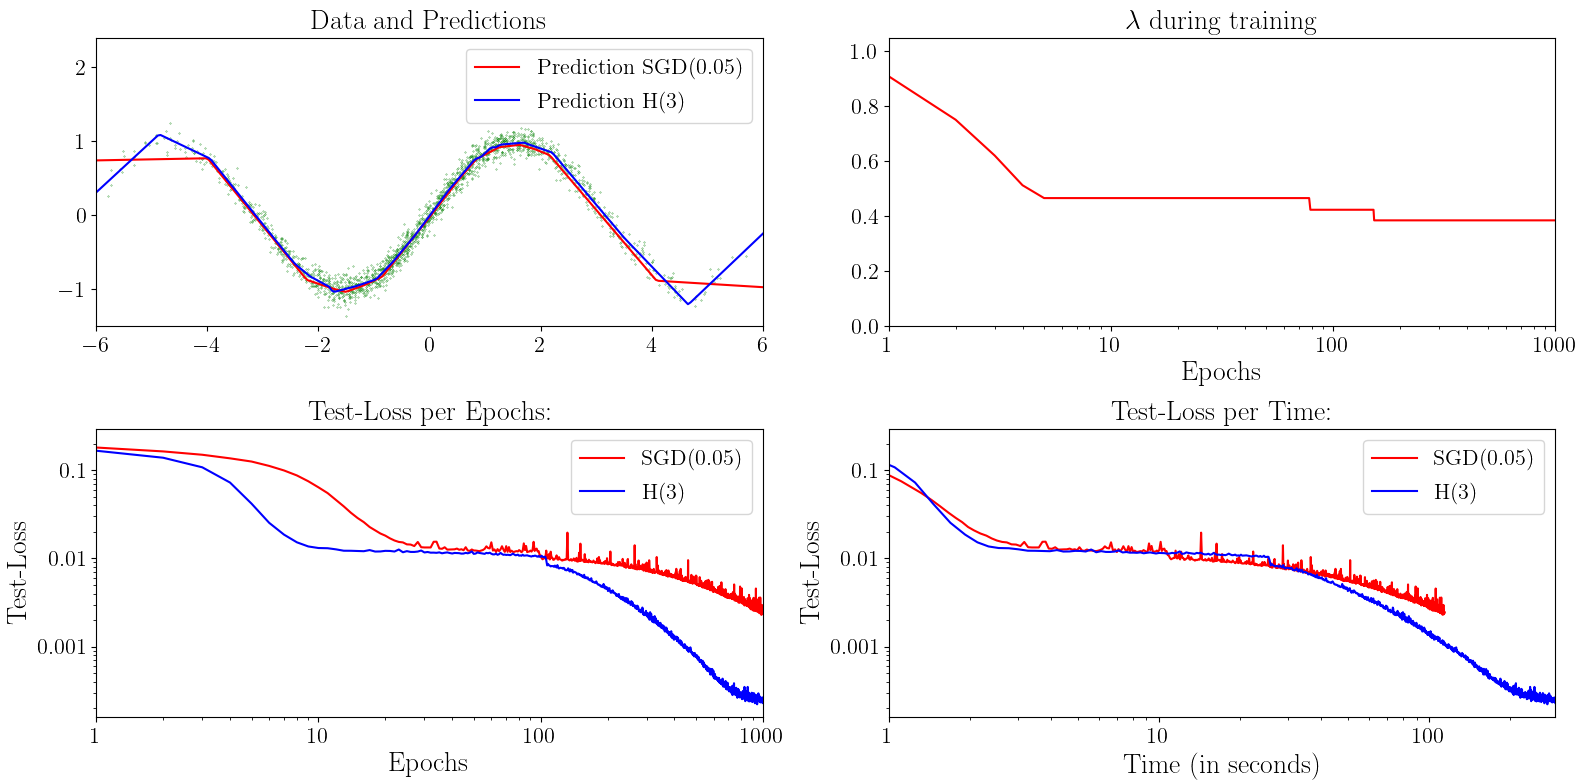
\includegraphics[width=\textwidth]{toy_005.png}
		\caption{Comparison of our Hessian-Free algorithm (3 CG-steps) with SGD (learningrate 0.05). For the $\lambda$-updates we chose $r=...$ for a stable optimization. Even if only a few samples were generated on the borders of the upper right graphic, Hessian-Free was able to fit the data well in contrast to SGD.}
		\label{fig2}
	\end{figure*}

	\subsection{MNIST}

	\noindent
	The MNIST database consists of grayscale images of handwritten digits from $0$ to $9$, with a resolution of $28\times28$ pixels. We flatten each image to a vector of size $784$ and divide by $255$, which transforms the data to $[0,1]^{784}$. The train data set consists of $60,000$ images. For validation we use the test data set with $10,000$ images.\\
	For our DNN we chose an architecture with one hidden layer with $800$ Neurons and ReLu activation function. The total Number of trainable Parameters is $636,010$.\\
	For stochastic gradient descent we chose as learning rate $\eta=0.1$ and batch size $M_{\mathrm{SGD}}=100$. We also tested $\eta=0.01$, $\eta=0.025$ and $\eta=0.3$ as well as $M_{\mathrm{SGD}}=250$, but it achieved worse results. \\
	The SGD benchmark for this model architecture with cross-entropy loss and previous softmax function without data pre-processing, distortion, weight-decay etc. is an error rate of $1.6\%$ on the test data set \href{https://en.wikipedia.org/wiki/MNIST_database}{(MNIST benchmark)} .
	It can be achieved by initially setting the learning rate to $\eta=0.005$ and multiplying it by $0.3$ every $100$ epochs. But convergence in this scenario is very slow.
	\begin{figure}[htbp]
		\centerline{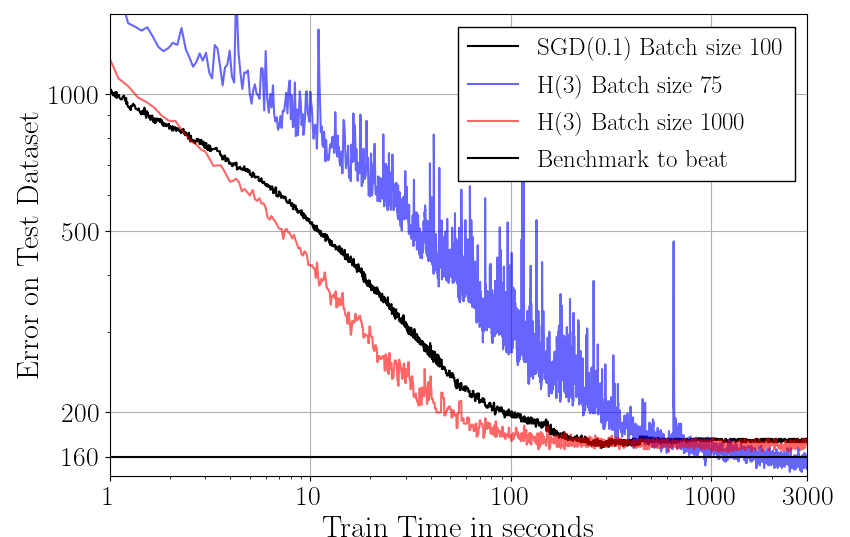
\includegraphics[scale=0.52]{Plot_Batch_size.png}}
		\caption{Comparison with SGD (black) and the effect of the batch size on performance. On the $y$-axis the total number of wrongly classified images on the whole test dataset is plotted. The corresponding train time to reach these result is plotted on the $x$-axis.}
		\label{fig3}
	\end{figure}
	\noindent
	We set the accuracy $\varepsilon=0.0005$ and the number of minimal PCG-steps to $3$. In this setting the PCG-method stops mostly after $6-10$ steps. A higher minimal PCG-step number e.g. $10$ does not lead to better performance, but significantly more time for one total update step is needed. Here PCG-method stops after $13-17$ steps.\\
	With a large batch size $(M_{\mathrm{HF}}=1000)$ the method converges faster than SGD with learningrate $\eta=0.1$ and $N=100.$ But generally SGD seems to converge more stable. After some time both methods tend to overfit on the train data. Here the total error on the train data converges to $0$, which prevents any improvement gains on the test dataset.\\
	With a smaller batch size $(M_{\mathrm{SGD}}=75)$ the method converges much slower than SGD with learningrate $\eta=0.1$ and also seems to be very unstable in comparison. But this instability prevents overfitting to the train data as the total error on the train data set never converges to $0$. At around $1000$ seconds the method passes SGD and at $2000$ seconds the method consistently beats the Benchmark. After around $3000$ seconds the best performance measured is a $1.46\%$ error rate but due to the stochasticity of mini batching can get as high as $1.62\%$ on some batches. Because minor performance gains are still noticeable it may be possible to achieve an even better error rate.
	Also the method becomes significantly more stable as the training progresses. Our results can are displayed in Fig. 3.\\
	We also tested the effect of using the preconditioned CG-Method rather than the vanilla CG-Method. This can be seen in Fig. 4, preconditioning leads to faster convergence to a slightly better level.


	\begin{figure}[htbp]
		\centerline{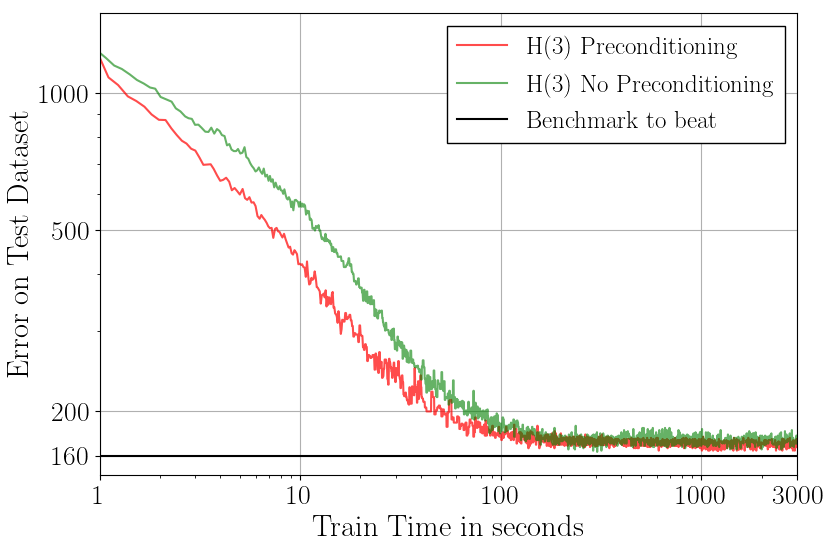
\includegraphics[scale=0.53]{Precond.png}}
		\caption{Comparison of the PCG-method and the CG-method. Without Preconditioning convergence is slower. (Tested with $M_{\mathrm{HF}}=100$)}
		\label{fig4}
	\end{figure}



	\section{Conclusion}
	...

	\section*{Acknowledgment}
	\noindent
	We want to thank the lecture assistant Florian Messerer for suggesting this topic for the project and giving us some sources to research.

	%	\bibitem{b1} M. Abadi, A. Agarwal, P. Barham, E. Brevdo,
	%Z. Chen, C. Citro, G. S. Corrado, A. Davis,
	%J. Dean, M. Devin, S. Ghemawat, I. Goodfellow,
	%A. Harp, G. Irving, M. Isard, R. Jozefowicz, Y. Jia,
	%L. Kaiser, M. Kudlur, J. Levenberg, D. Mané, M. Schuster,
	%R. Monga, S. Moore, D. Murray, C. Olah, J. Shlens,
	%B. Steiner, I. Sutskever, K. Talwar, P. Tucker,
	%V. Vanhoucke, V. Vasudevan, F. Viégas,
	%O. Vinyals, P. Warden, M. Wattenberg, M. Wicke,
	%Y. Yu, and X. Zheng,
	%TensorFlow: Large-scale machine learning on heterogeneous systems,
	%2015. Software available from tensorflow.org.


	\begin{thebibliography}{00}
		\bibitem{b1} M. Abadi, A. Agarwal, P. Barham, E. Brevdo,
		Z. Chen, C. Citro, G. S. Corrado, A. Davis,
		J. Dean, M. Devin, S. Ghemawat, I. Goodfellow,
		A. Harp, G. Irving, M. Isard, R. Jozefowicz, Y. Jia,
		L. Kaiser, M. Kudlur, J. Levenberg, D. Mané, M. Schuster,
		R. Monga, S. Moore, D. Murray, C. Olah, J. Shlens,
		B. Steiner, I. Sutskever, K. Talwar, P. Tucker,
		V. Vanhoucke, V. Vasudevan, F. Viégas,
		O. Vinyals, P. Warden, M. Wattenberg, M. Wicke,
		Y. Yu, and X. Zheng,
		TensorFlow: Large-scale machine learning on heterogeneous systems,
		2015. Software available from tensorflow.org.
		\bibitem{b2} M. Diehl, "Lecture Notes on Numerical Optimization (Preliminary Draft)", Albert Ludwigs University of Freiburg, September 29, 2017
		\bibitem{b3} M. Gargiani, A. Zanelli, M. Diehl, F. Hutter, "On the Promise of the Stochastic Generalized Gauss-Newton Method for Training DNNs",  arXiv:2006.02409v4, June 9, 2020
		\bibitem{b4} J. Martens, "Deep learning via Hessian-free optimization", University of Toronto, Ontario, M5S 1A1, Canada, 2010
		\bibitem{b5} J. Martens, "New Insights and Perspectives on the Natural Gradient Method", Jurnal of Machine Learning Research 21, arXiv:1412.1193v11, September 19, 2020
		\bibitem{b6} J. Martens, I. Sutskever, "Training Deep and Recurrent Networks with Hessian-Free Optimization", In: G. Montavon, G.B. Orr, KR. Müller (eds), Neural Networks: Tricks of the Trade. Lecture Notes in Computer Science, vol 7700. Springer, Berlin, Heidelberg, 2012
		\bibitem{b7} B. A. Pearlmutta, "Fast Exact Multiplication by the Hessian", Neural Computation, June 9, 1993
		\bibitem{b8} N. N. Schraudolph, "Fast Curvature Matrix-Vector Products for Second-Order
		Gradient Descent", Neural Computation, August 2002
		\bibitem{b9} G. Van Rossum, F. L. Drake, Python 3 Reference Manual. Scotts Valley, CA: CreateSpace, 2009
	\end{thebibliography}
\end{document}
